% Guillaume Fraux PhD thesis -- (C) 2019
% Distributed under CC-BY-SA-NC license 4.0
% Creative Commons Attribution-NonCommercial-ShareAlike 4.0 International
\documentclass[thesis]{subfiles}

\begin{document}

\chapter{Adsorption and intrusion in nanoporous materials}
\vspace*{-1\baselineskip}
\section{Nanoporous materials}

Porous materials are materials which present a structural porosity, such that their
tri-dimensional structure shows cavities called \emph{pores}. This network
of pores can vary in homogeneity and regularity, creating a wide variety of
porous materials. They all have in common a high specific surface area, which is
the accessible internal surface by grams of the material --- up to thousands of
square meters by gram of material\cite{Farha2012} in the most extreme cases.
This very high specific surface area of porous materials is exploited in a
number of important industrial applications, especially in the domains of
adsorption and catalysis. For example, porous materials are used to separate
gases in mixtures as molecular sieves; to filter and remove heavy metals from
water; or in heterogeneous catalysis in oil refineries by the cracking process.

The International Union for Pure and Applied Chemistry (IUPAC) recommends to
classify porous materials in three groups, depending on the size of the
pores\cite{Rouquerol1994}. First are the \emph{microporous} solids, where the
pores are less than \SI{2}{nm} in diameter. Then we find the \emph{mesoporous}
solids with pore diameter between 2 and \SI{50}{nm}. Porous solids with pores
larger than \SI{50}{nm} are called \emph{macroporous} solids. Microporous and
mesoporous solids are often grouped together as \emph{nanoporous} solids, where
the size of pores does not exceed \SI{50}{nm}.

\begin{figure}[ht]
    \centering
    \raisebox{-0.5\height}{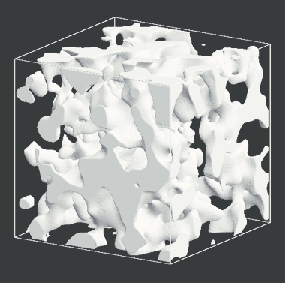
\includegraphics[width=0.3\textwidth]{figures/cited/porous-vycor}}
    \hfill
    \raisebox{-0.5\height}{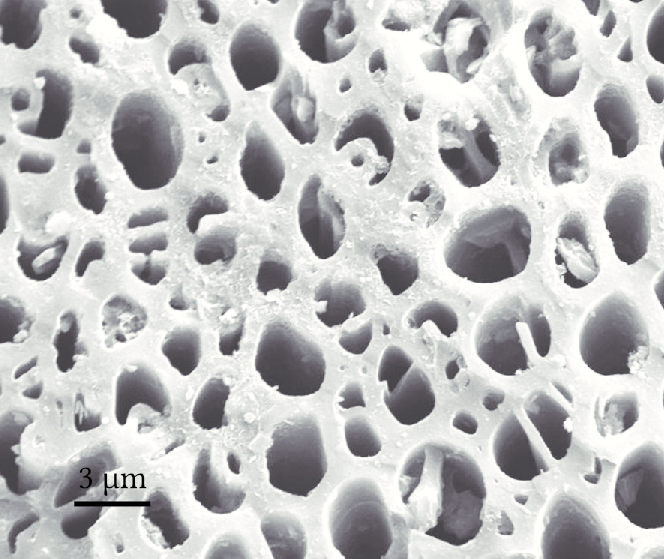
\includegraphics[width=0.3\textwidth]{figures/cited/porous-carbon}}
    \hfill
    \raisebox{-0.5\height}{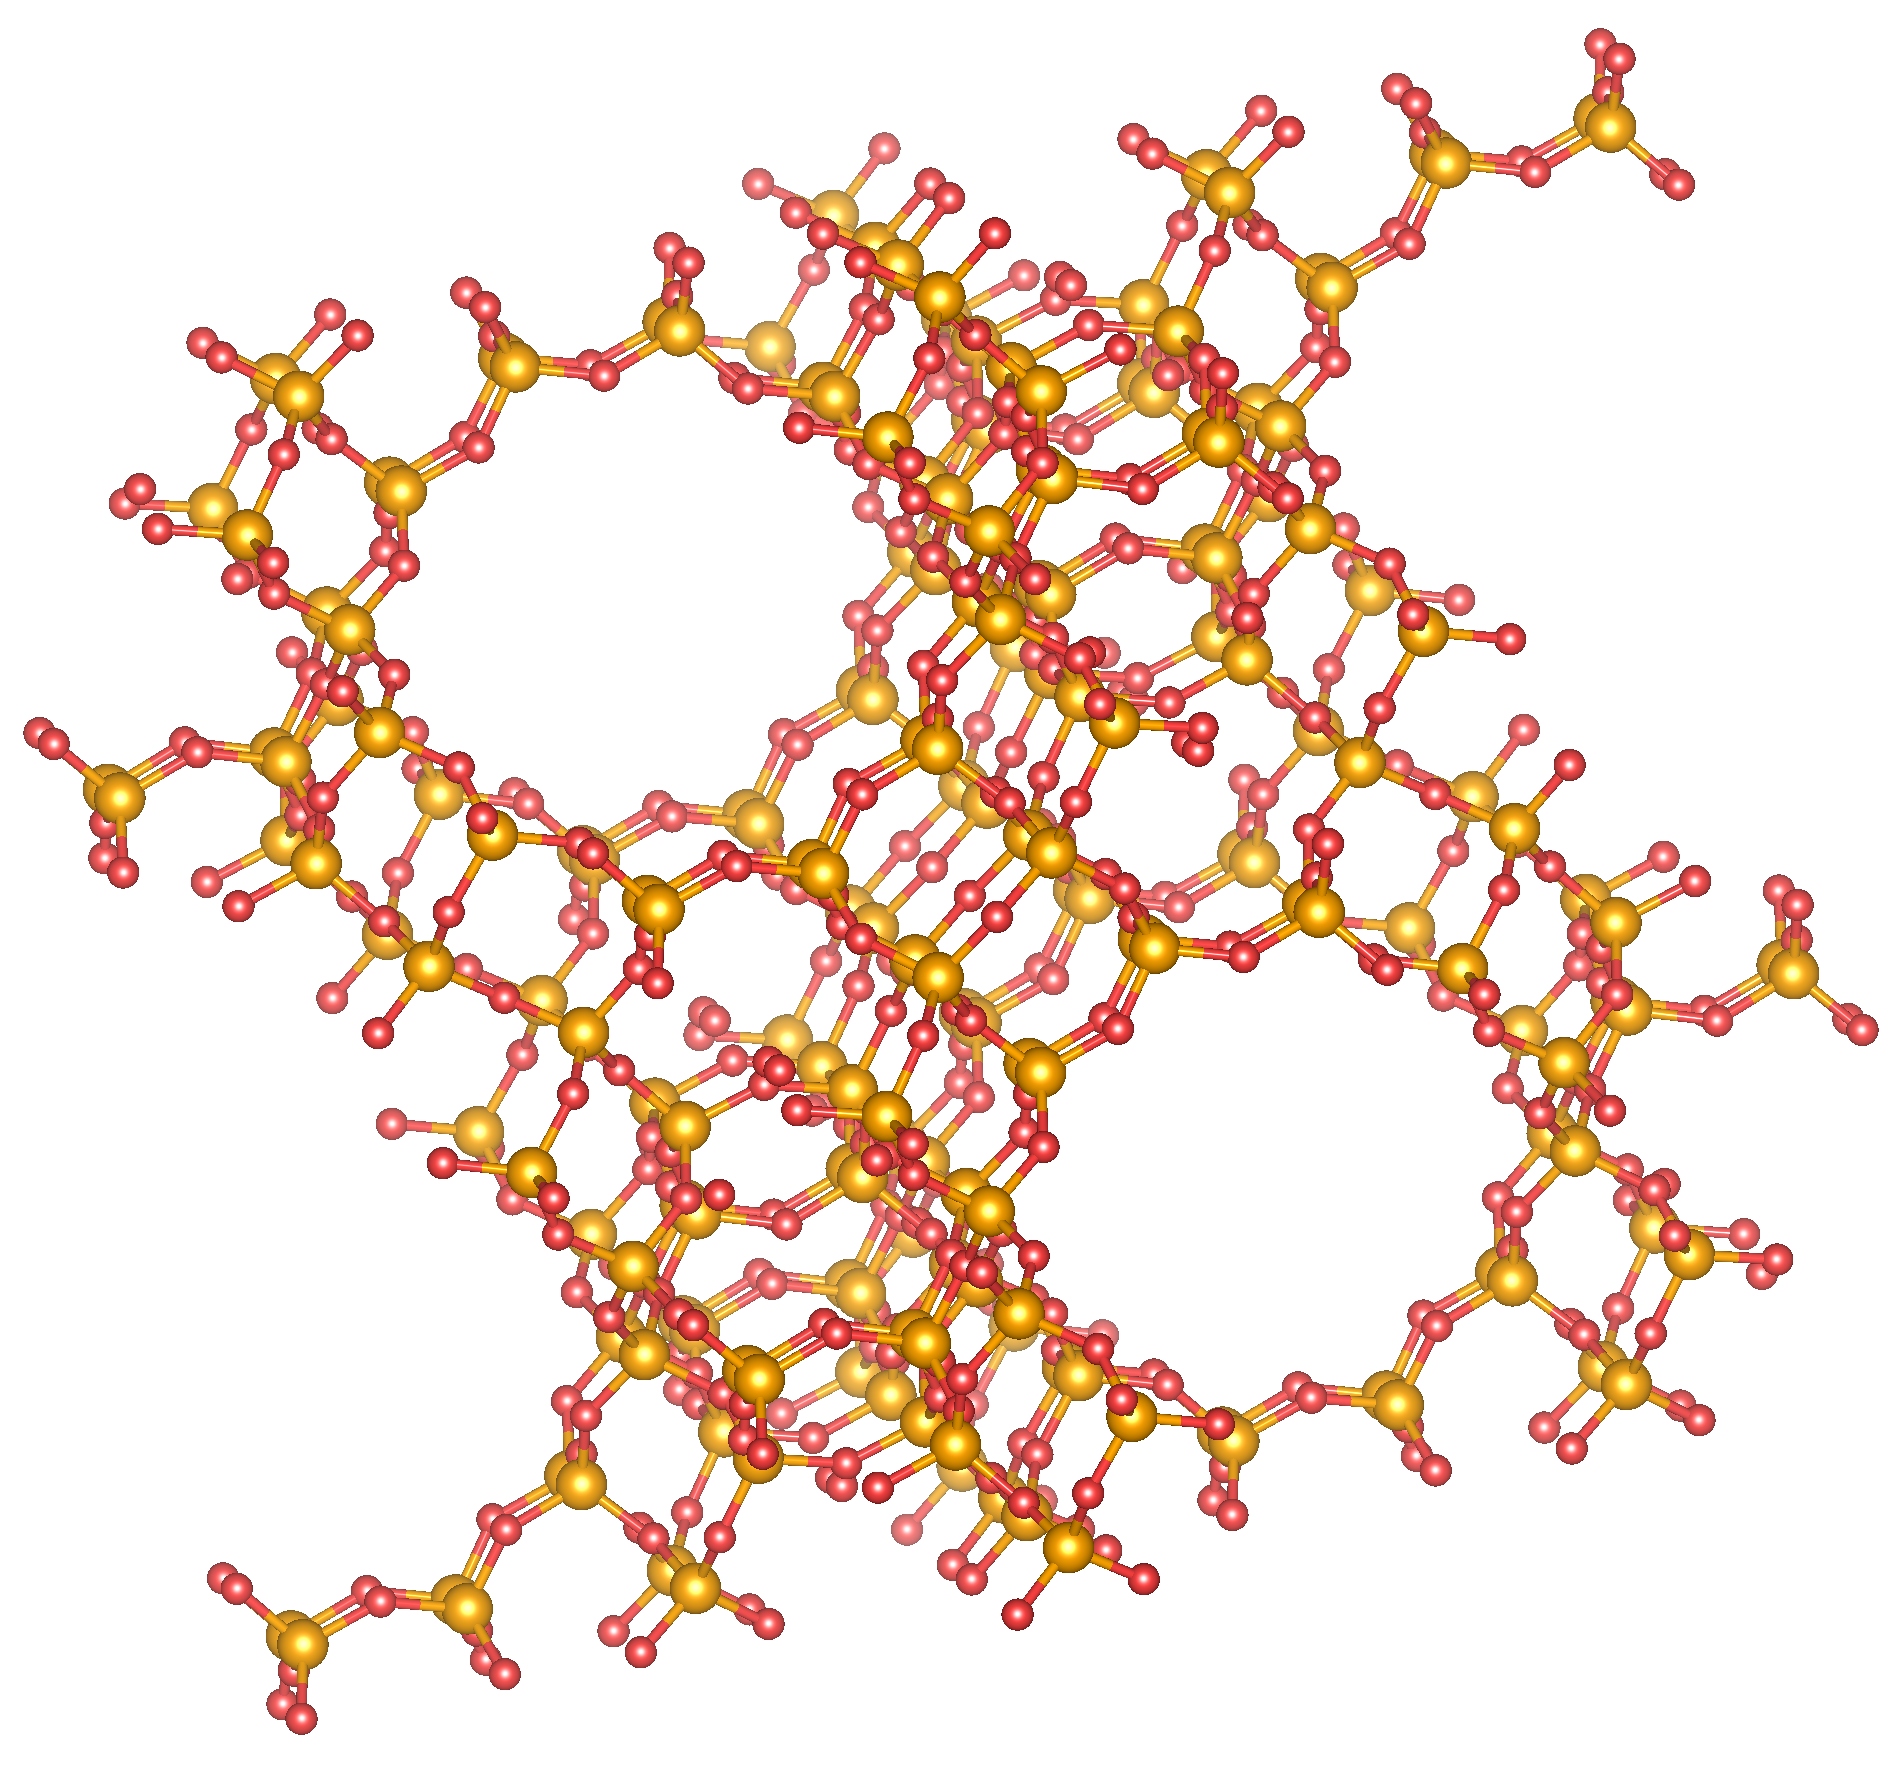
\includegraphics[width=0.3\textwidth]{figures/cited/porous-faujasite}}
    \caption{Three examples of porous materials. The left image is a
    representation of a vycor glass (disordered) (Reprinted with permission from
    reference~\cite{Levitz2003}, copyright (2003) Elsevier); the middle is a
    scanning electron microscope image of activated carbon (ordered but non
    crystalline)\cite{Das2015}; and right is the crystalline structure of the
    zeolite faujasite.}
    \label{fig:porous-examples}
\end{figure}

Porous materials are also classified depending on their structural regularity,
from highly regular crystalline materials such as zeolites and
\emph{Metal--Organic Frameworks} (MOFs) showing a periodic organization of their
atoms; to regular porous materials such as clays and carbon nanotubes, where the
porosity is well defined but does not present long-distance ordering. Finally,
there also exist amorphous porous materials, which have a wide distribution of
pore sizes and shapes, and no periodicity. Examples in this latter class are
vycor glasses, silica glasses, or aerogels. Three examples of porous solids with
different pore size and regularity are presented in figure~\ref{fig:porous-examples}.

A final distinction we can make among porous materials is that of their chemical
nature. They are usually classified as either organic or inorganic materials.
The former contain materials built around carbon atoms, such as carbon
nanotubes, microporous carbons, or porous organic polymers. The latter class has
historically been the widest one, containing materials such as porous oxides,
alumino-silicates, sulfur compounds or alumino-phosphates. In the last few
decades, we have seen blooming a new class of materials, with a hybrid
inorganic-organic composition. This new family contains materials such as
organo-silicic crystals, and metal--organic frameworks, which have been the main
subject of study in my PhD.

During my PhD, I studied hybrid inorganic-organic crystalline nanoporous
materials, and in particular flexible ones. In the next sections, I will
describe zeolites as the conventional example of crystalline porous materials,
and MOFs as the relatively new class of hybrid inorganic-organic porous
materials. I will also present the \emph{Zeolitic Imidazolate Framework} (ZIF)
family of MOFs, which are MOFs with a zeolitic topology.

\subsection{Zeolites}

Zeolites were named by the Swedish mineralogist Axel Fredrik Cronsted in
1756\cite{Ferey2001} from the Greek \textgreek{ζέω} (zéō), meaning "to boil" and
\textgreek{λίθος} (líthos), meaning "stone". He observed that when heating a
fragment of stilbite mineral to 150°C, the stone started to cover itself with
small bubbles, as if the stone was starting to boil --- we now understand it as
the desorption of water from inside the zeolite's pores. In the following decades,
around twenty additional natural zeolites were discovered. In 1862, French
chemist Henri Sainte-Claire Deville, created the first artificial analog to
zeolites, but it was only in 1930 that Linus Pauling resolved the structure of
zeolites using X-ray diffraction. Today, 234 unique zeolite frameworks have been
identified, and we know over 65 naturally occurring zeolite frameworks according
to the International Zeolite Association\cite{iza-website}.

\subsubsection{Structure and composition}

Zeolites are porous crystalline alumino-silicates, with a structure built around
a regular arrangement of \ce{SiO4} or \ce{AlO4} tetrahedra linked together by
their vertices as represented in figure~\ref{fig:zeolite-building-block}. The
porous network created by these tetrahedra is very different from one zeolite to
another, resulting in a wide variety of materials and properties. For examples,
the pores can be linear, spherical or in a zigzag disposition; connected
together through windows or independents. The International Zeolite
Association\cite{iza-website} gives a three letter code such as LTA, FAU or SOD
to each experimental crystalline structure. It is however mathematically
possible to generate an infinite number of crystalline structures using
tetrahedra as a building block, and there are databases of hypothetical zeolites
with more than 2 million different frameworks\cite{hypothetical-zeolites}.

\begin{figure}[ht]
    \centering
    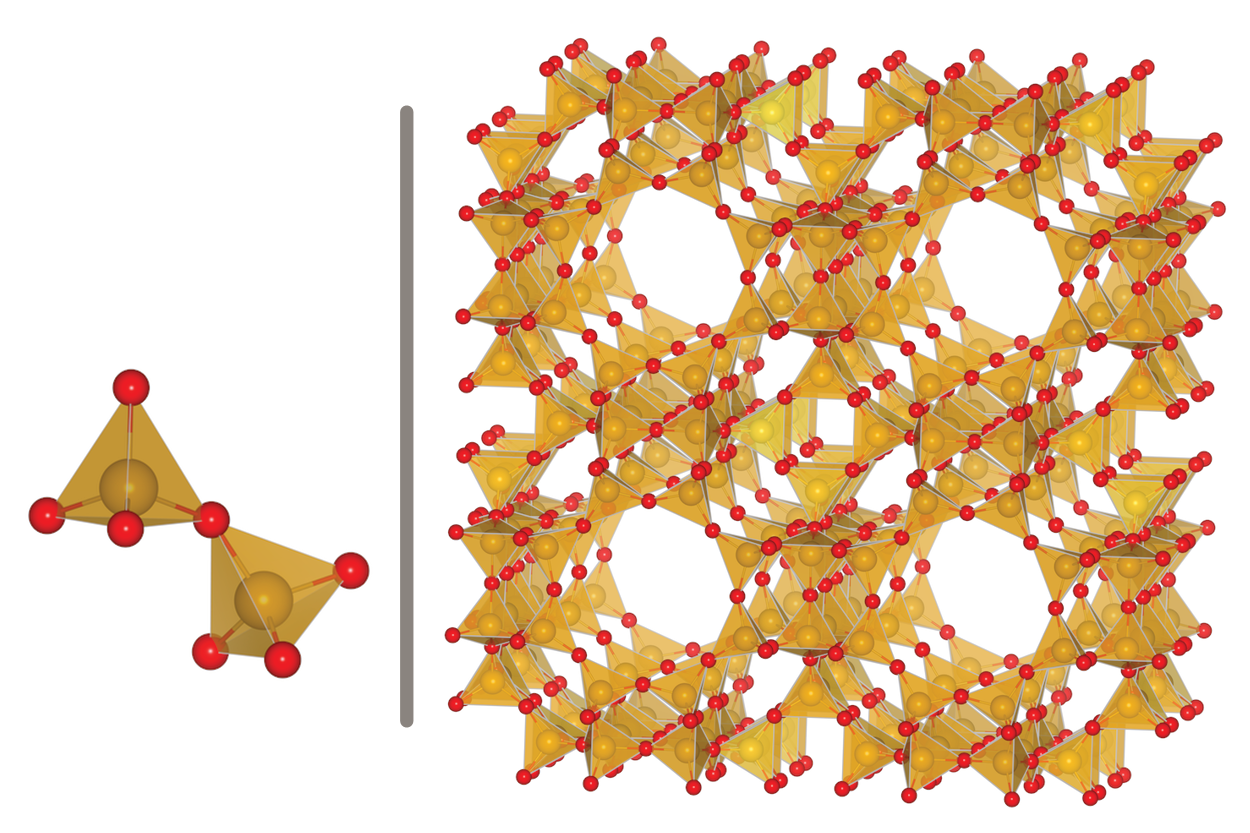
\includegraphics[width=0.7\textwidth]{figures/images/zeolite-building-blocks}
    \caption{Two \ce{SiO4} tetrahedra on the right, and the structure of zeolite
    LTA on the left. Si atoms are in yellow and oxygen atoms in red.}
    \label{fig:zeolite-building-block}
\end{figure}

While pure-silica zeolites (\ce{SiO2} polymorphs) are neutral, each aluminum
atom in the structure introduces a negative charge as silicon is usually in the
+IV oxidation state while aluminum is in the +III state. These charges are
compensated in the material by a counter ion such as sodium \ce{Na+}, potassium
\ce{K+}, calcium \ce{Ca^{2+}} or barium \ce{Ba^{2+}}. Each zeolite topology thus
defines a family of materials with varying chemical composition. The general
chemical formula for a zeolite is $\text{M}_{x/m}\, \text{Al}_x\,
\text{Si}_{\,1-x}\, \text{O}_2$, possibly with several different metal cation M.
The Si/Al ratio can vary from 1 for structures with the most aluminum atoms to
infinity for pure silica zeolites, also called \emph{zeosil}. Each new aluminum
atom replacing a silicon atom is accompanied by a cation to ensure the overall
charge neutrality. The presence of these cations contributes to the remarkable
adsorption and catalysis properties of zeolites. Zeolites are used in industrial
processes for ions exchange through their extra cations; catalysis through their
high specific surface area and acido-basic properties; molecular sieves through
the multiples pores sizes and tunable properties.

\newpage
\subsection{Metal--Organic Frameworks}

Metal--organic frameworks are a more recent class of crystalline nanoporous
materials. The first works on these materials were made in the 90s by Richard
Robson and collaborators\cite{Abrahams1991, Robson2008}, but the systematic
study of these materials only started in the 2000s. In 1999, the group of Omar
Yaghi created MOF-5\cite{Li1999}, a MOF with large permanent porosity
(\SI{15}{\AA} in diameter for the largest cavity) and chemical tunability,
sparking interest in the international research community for these materials.
Since then, the field of MOF has been developing exponentially, both in terms of
the number of publications and in terms of number of structures reported in the
literature. Figures~\ref{fig:number-of-mofs} shows the growth of the number of
structures in the Cambridge Structural Database, with a doubling time of 3.9
years for three-dimensional MOFs.

\begin{figure}[ht]
    \centering
    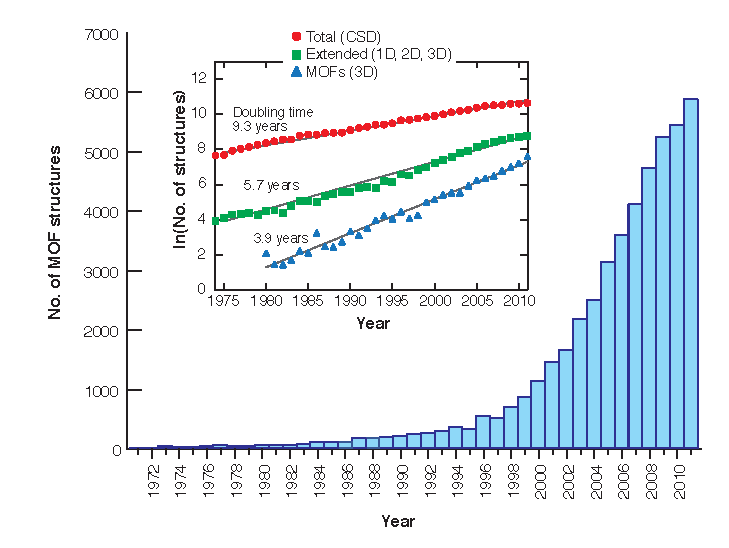
\includegraphics[width=0.8\textwidth]{figures/cited/number-of-mofs}
    \caption{Number of MOF structures in the Cambridge Structural Database
    showing an exponential growth. Reprinted with permission from AAAS,
    reference~\cite{Furukawa2013}.}
    \label{fig:number-of-mofs}
\end{figure}

Materials in the MOF family are built around metallic centers, connected by
organic linkers, assembled into nano- or mesoporous crystalline structures (see
figure~\ref{fig:mof-building-blocks}). Compared to zeolites, they can be
synthesized in a solvent at lower temperatures (from ambient temperature to
200°C), by mixing metallic salts and organic linkers. Due to the presence of
these organic linkers, MOFs have smaller thermal stability (up to 400°C)
compared to the inorganic zeolites that can withstand up to 1000°C.
Nevertheless, this reduced stability is made up for by the incredible
adaptability of the MOFs. By combining the variety of linker-metal coordination chemistry
with the adaptability of organic chemistry, they offer a huge number of
different structures, and can be tuned for specific applications by changing
linkers and/or metal centers. Figure~\ref{fig:mof-different-linkers} presents an
example of how the shape and size of the pores can be adapted by changing the
linker used. Furthermore, compared to zeolites which present a rigid crystalline
structure, some MOFs grouped together under the name \emph{Soft Porous
Crystals}\cite{Horike2009} have extraordinary structural flexibility in
response to external stimuli\cite{Kitagawa2005, Bradshaw2005, Coudert2015}.

\begin{figure}[p]
    \centering
    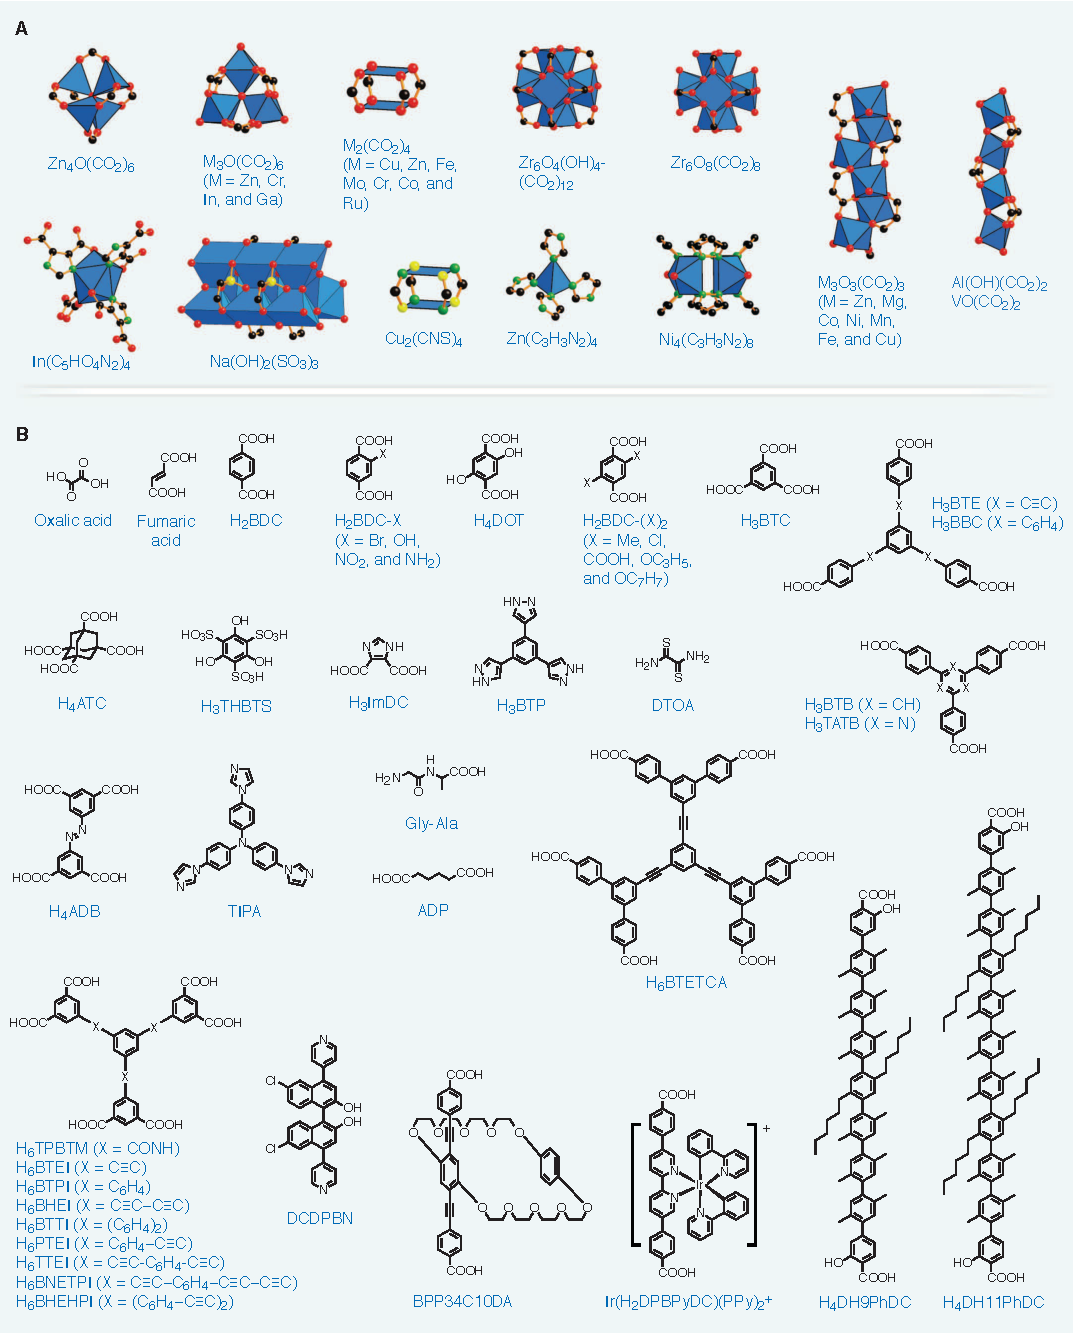
\includegraphics[width=\textwidth]{figures/cited/mof-building-blocks}
    \caption{Examples of inorganic clusters (A) and organic linkers (B) used in
    MOF synthesis. Reprinted with permission from AAAS, reference~\cite{Furukawa2013}.}
    \label{fig:mof-building-blocks}
\end{figure}

\afterpage{\clearpage}

\subsubsection{High diversity of structures}

One of the main advantage of MOFs over other porous materials such as zeolites
or activated carbons is the diversity of structures that can be built from the
different available inorganic clusters and organic linkers (see
figure~\ref{fig:mof-building-blocks}). With all the versatility provided by the
coordination and organic chemistry, one is only limited by the thermodynamic and
chemical stability of the structures obtained, and by the existence of a
synthetic route to generate the porous polymorphs of interest, when another
phase might be more stable. This diversity of structure gave rise to a
\emph{design to applications} approach, where one aims at producing the best
structure for a given functionality. For example, researchers have reported MOFs
with the highest methane\cite{Tian2017} or hydrogen\cite{Oh2017} uptakes until
now.

\begin{figure}[ht]
    \centering
    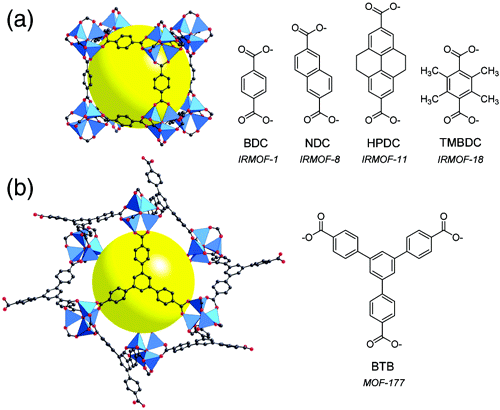
\includegraphics[width=0.7\textwidth]{figures/cited/mof-different-linker}
    \caption{Examples of two MOFs built with a zinc oxide cluster with the same
    coordination geometry. (a) Structure of MOF-5, made with a linear linker.
    (b) Structure of MOF-177, made with a trigonal linker. Reprinted with
    permission from reference~\cite{Rowsell2004}, copyright (2004) American
    Chemical Society.}
    \label{fig:mof-different-linkers}
\end{figure}

They are two different approaches used to create new MOF structures. The first
one is to use linkers and metallic centers with different connectivity, such as
the ones shown in figure~\ref{fig:mof-different-linkers}. Most of the linkers
used in MOF present either carboxylate or nitrogen organic functions that bind
the metals. Using a linker with a different number of these functions or a metal
center with different oxidation degree will create a new structure. The second
way to create a new structure is by changing the chemical structure of the
linker, while keeping the number and positions of binding functions intact. The
resulting structures are said to be \emph{isoreticular}, \ie they share the same
topology or net.

\subsection{Zeolitic Imidazolate Frameworks}

\begin{figure}[ht]
    \centering
    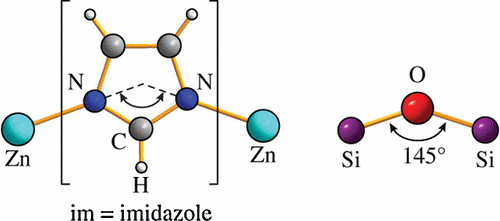
\includegraphics[width=0.7\textwidth]{figures/images/zeolite-to-zif}
    \caption{Illustration of the analogy between ZIFs and zeolite coordination.}
    \label{fig:zeolite-to-zif}
\end{figure}

\emph{Zeolitic Imidazolate Framework} or ZIFs are a family of MOFs built around
tetravalent \ce{M^{2+}} metal centers such as Fe, Co, Zn, Cd or Cu; linked
together by imidazolate or functionalized imidazolate linkers. They present the
same possible topologies as zeolites, with metal(imidazolate)$_2$ building
blocks taking the role of \ce{SiO2} --- as illustrated in
figure~\ref{fig:zeolite-to-zif}. The first ZIFs (ZIF-1 to ZIF-12) were
synthesized in 2006\cite{Park2006}, and found to be more resistant to water and
heat that typical MOFs, which made them interesting for commercial applications.
This higher stability is due to the relatively strong metal--imidazolate
coordination bond.

\begin{figure}[b]
    \centering
    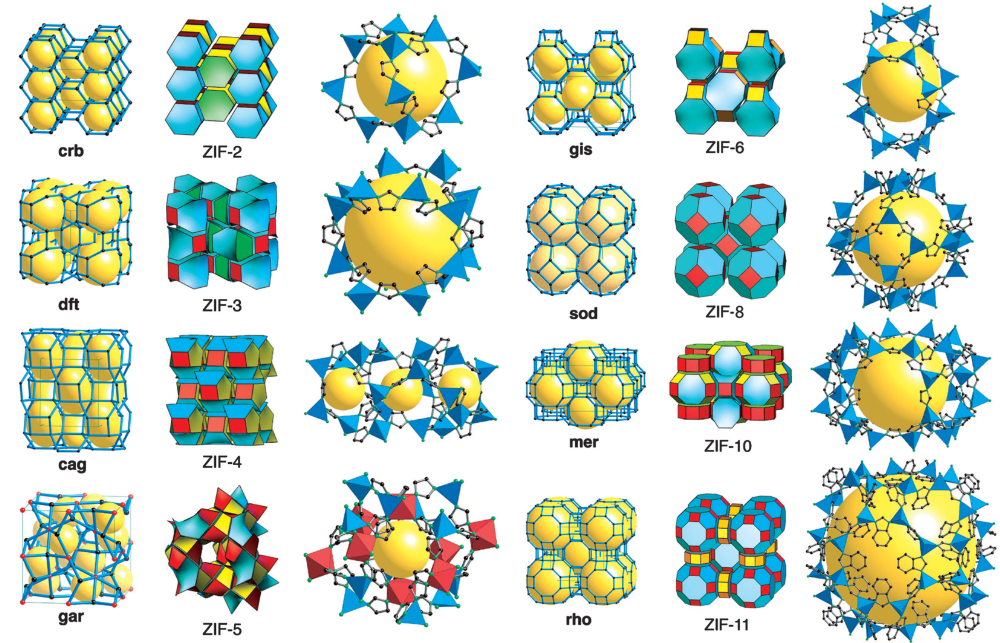
\includegraphics[width=\textwidth]{figures/cited/zif-examples}
    \caption{Examples of ZIF structures. From left to right are the crystalline
    structure of a zeolite with the same topology, the crystalline structure of
    the ZIF and the biggest sphere inside the cages. Reprinted from
    reference~\cite{Park2006}, copyright (2006) The National Academy of
    Sciences of the USA.}
    \label{fig:zif-examples}
\end{figure}

\ZIF8 is the member of the ZIF family which I worked on specifically during my
PhD. It uses 2-methylimidazolate (mim) as a linker, and \ce{Zn^2+} as its
metallic centers. \ZIF8 has formula \ce{Zn(mim)2} and adopts the sodalite
(\textbf{sod}) topology. In this topology, large quasi-spherical pores
corresponding to the sodalite cages are connected by windows formed by 6 and 4
zinc atoms. In \ZIF8, the 4 members windows are too small for any molecules to
go through, and all of the connectivity of the pore space happens through the 6
members windows. I also studied materials derived from \ZIF8, where the methyl
group of the linker is replaced by halogens such as chlorine or bromide. The
corresponding studies are presented in sections~\ref{sec:zif8x}
and~\ref{sec:zif8-intrusion}.

\newpage
\subsection{Structural flexibility}

In 1998, Susumu Kitagawa proposed a classification of MOFs in three
categories\cite{Horike2009} depending on their behavior with respect to
molecule adsorption and desorption. The first category of materials has a
non-permanent porosity, in the sense that if we remove the solvent molecules
from the structure after the synthesis, the material collapses. The second
category regroups materials that have a strong enough crystalline structure and
keep the same porosity during adsorption and desorption. They are essentially
rigid, and generally present a very good mechanical and thermal stability. The
last category contains materials that retain porosity when the synthesis solvent
is removed, but may deform and change shape during adsorption. Materials in this
last category are called \emph{Soft Porous Crystal}, and have a flexible,
dynamic structure that can change under external stimuli such as mechanical
pressure, adsorption, temperature, or even exposure to light\cite{Kitagawa2005,
Coudert2015}.

\begin{figure}[ht]
    \centering
    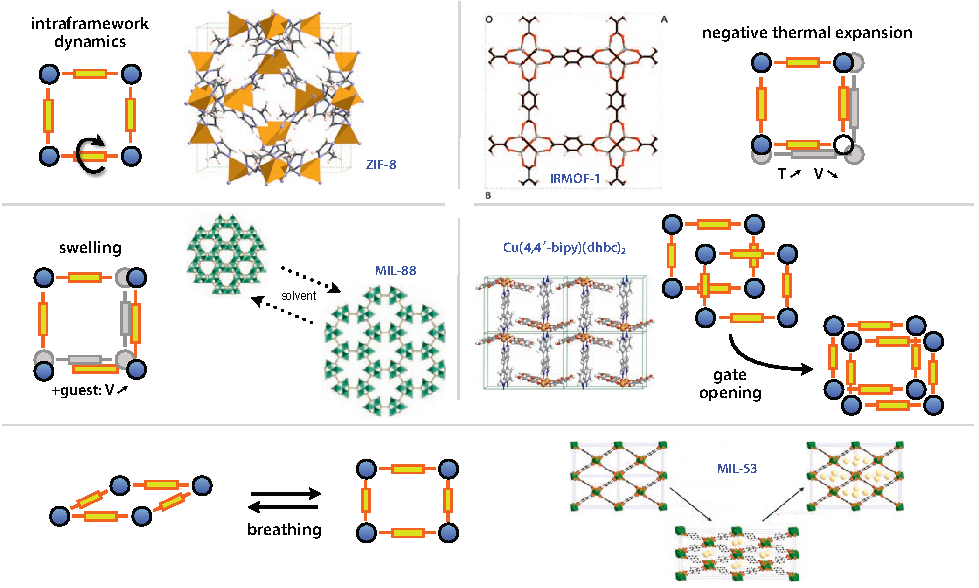
\includegraphics[width=\textwidth]{figures/cited/mof-flexibility}
    \caption{Illustration of the main flexibility modes of MOFs: linkers
    rotation, thermal expansion, swelling, gate opening and breathing. Reprinted
    with permission from reference~\cite{Coudert2011}, copyright (2011) Wiley.}
    \label{fig:mof-flexibility}
\end{figure}

This flexibility is inherent to the hybrid organic-inorganic nature of MOFs.
Indeed, their structure is based on both strong covalent bonds inside the
organic linkers, and weaker bonds such as coordination bonds, $\pi$-stacking of
linkers, hydrogen bonds, \etc These weaker bonds can vary locally in length or
orientation, inducing large scale deformations of the materials. Possible
deformation modes for MOFs are represented in figure~\ref{fig:mof-flexibility}.
All MOFs are flexible to some extent through local deformations, such as linkers
rotation, this type of flexibility happening without any global framework
deformations. The other types of flexibility only occur in specific materials.
For example, we observe in some materials a volume contraction as they heat
up, \ie a called \emph{negative thermal expansion}\cite{Dubbeldam2007}.

In soft porous crystal, we additionally observe large scale deformations of the
structure. For some materials, the whole structure will swell in presence of a
solvent. For example, the volume of MOFs of the MIL-88 family can grow by more
than 200\% of the initial volume in presence of lutidine\cite{Serre2007}. Other
MOFs present multiple stable phases, and can switch from one phase to another
under external stimuli. The \emph{gate opening} phenomenon is one of such
transitions, between an initially non-porous structure to a more open and more
porous structure through the movement of linkers or the displacement of a
sub-network. Materials from the MIL-53 family present two transitions, from an
open to a close-pore phase, and then back to an open-pore phase\cite{Serre2002}
under continuous gas loading increase, creating a \emph{breathing}-like
behavior.

\subsection{Industrial applications}

Zeolites enjoy a wide range of applications, from air separation using pressure
swing adsorption\cite{Rege1997}, catalysis in oil refining\cite{Primo2014},
wastewater cleaning and heavy metal removal\cite{Curkovi1997}, capture of
radioactive particles\cite{Borai2009}, molecular sieve\cite{Flanigen1978}, and
even laundry detergent\cite{Karge1989}. Each year, almost 3 million tonnes of
zeolites are produced or extracted for these applications. MOFs are still
relatively new, and don't enjoy as many commercial and industrial applications
as zeolites yet. One of the obstacles to wider usage of MOFs is their price,
as they can be a hundred times more expensive than zeolites. In the following, I
will give examples of potential applications of MOFs in various fields.

\subsubsection{Gas separation, purification, and storage}

Gas separation and purification processes are at the root of the chemical
industry, either generating small carbon chain molecules from oil and natural
gas, separating oxygen from nitrogen in the air, or \ce{CO2} from \ce{H2} during
ammonia production. Current best estimates indicate that gas separation accounts
for 10-15\% of the energy consumed globally\cite{Sholl2016}. Furthermore, when
faced with climate change resulting from continually-increasing anthropogenic
\ce{CO2} emissions, optimization of storage and separation processes is
increasingly critical. There are nowadays multiple techniques used for gas
separation using cryogenic separation, liquid phase adsorption or gas phase
adsorption. Few techniques based on gas phase adsorption are illustrated in
figure~\ref{fig:adsorption-processes}.

\begin{figure}[ht]
    \centering
    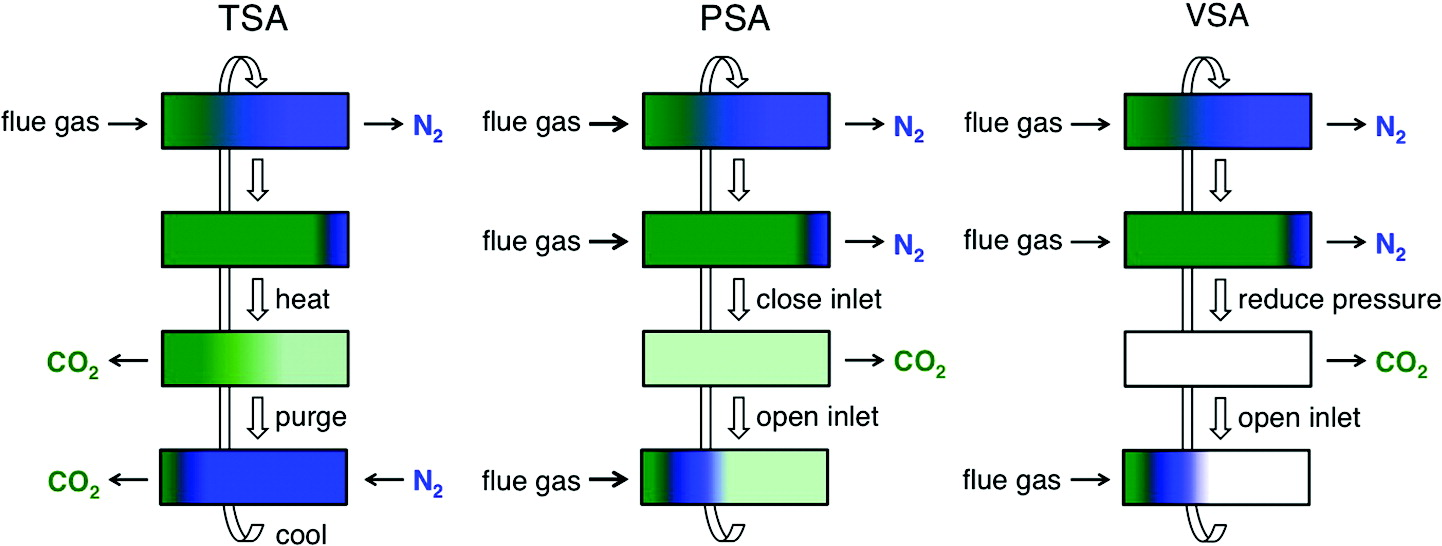
\includegraphics[width=\textwidth]{figures/cited/adsorption-processes}
    \caption{Schematic diagrams of temperature swing adsorption (TSA),
    pressure swing adsorption (PSA), and vacuum swing adsorption (VSA)
    processes for regenerating solid adsorbent in a fixed-bed column.
    Reprinted with permission from reference~\cite{Sumida2011}, copyright
    (2011) American Chemical Society.}
    \label{fig:adsorption-processes}
\end{figure}

As porous materials with huge specific surface area, MOFs look like ideal
candidates for any application involving gas adsorption. Separating gases by
adsorption requires different interactions between the porous material and the
different adsorbates. These interactions can be tuned in MOFs by changing the
linkers and modifying the pores size, shape and chemical properties. During gas
purification, one chemical species is present in majority (the gas to purify) and
we try to remove the remaining impurities. For example, HKUST-1 (a MOF with
formula \ce{Cu3(btc)2}) turned out to be very efficient to remove sulfur
compounds such as tetrahydrothiphene and thiophene from natural gas, thanks to
the formation of a \ce{Cu-S} bond\cite{Mueller2006}. It was able to adsorb
\SI{70}{g} of tetrahydrothiphene by liter of material, which is noticeably
better than the standard materials used in the industry (less than \SI{10}{g/L}
for activated carbons).

Considering gas storage, an emerging application is the storage of hydrogen gas
for energy generation and automobile transportation. Historically, hydrogen has
been stored through liquefaction or compression in bottles and tanks, but these
approaches have security and cost issues. MOFs are interesting as safer media
for gas storage because they are able to pack the hydrogen molecules densely at
a lower pressure. For example, \ce{Ni2(\textit{m}-dobdc)} is one of the current
best candidate for \ce{H2} storage, able to adsorb \SI{11}{g/L} of \ce{H2} at
ambient temperature, and up to \SI{23}{g/L} via a temperature swing from -75°C
to 25°C\cite{Kapelewski2018}.

\subsubsection{Heterogeneous catalysis}

\begin{figure}[ht]
    \centering
    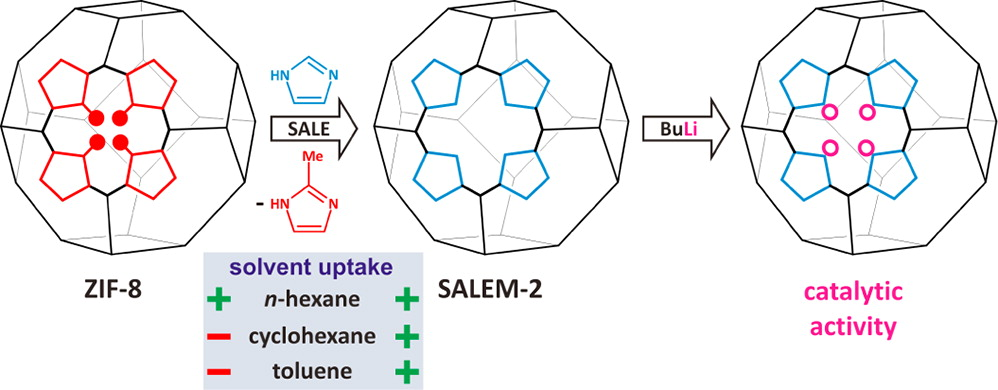
\includegraphics[width=\textwidth]{figures/cited/zif8-to-salem2}
    \caption{Post-synthetic modifications of \ZIF8 to synthesize SALEM-2 and
    obtain catalytic activity. Reprinted with permission from
    reference~\cite{Karagiaridi2012}, copyright (2012) American Chemical Society.}
    \label{fig:zif8-to-salem2}
\end{figure}

Heterogeneous catalysis is used in numerous industrial processes. The
selectivity of these catalytic processes is often based on the shape and size of
the reacting species, hence the interest in using catalysts with a regular and
uniform porosity. Porous crystalline materials are especially interesting in
this regard. Moreover, since catalysts can be re-used, and only small
quantities of them are needed, the advantages of MOFs can offset their cost. The
possibilities to create chiral MOFs using enantiomerically pure linkers, or
conformational chirality\cite{Tshabang2018} also opens the way to asymmetric
catalysis.

A first strategy for using MOFs as catalysts involves the metallic centers,
which can have a catalytic activity of their own. For example, MIL-100(Fe) and
MIL-100(Cr) have an interesting activity for the Friedel--Craft benzylation
reaction, used for the production of linear alkyl-benzene; surpassing the
activity of the HBEA and HY zeolites traditionally used\cite{Horcajada2007}.
HKUST-1 MOF can be activated after the synthesis by removing an apical water
molecule, creating a very reactive Lewis acid site which can be used for
cyanosilylation reactions\cite{Schlichte2004}.

Another approach for adding catalytic activity to MOFs entails adding functional
groups to the linkers with the desired activity. For example, SALEM-2 can be
activated with $n$-butyllithium and exhibits a strong Brønsted base catalytic
activity\cite{Karagiaridi2012} (see figure~\ref{fig:zif8-to-salem2}). Around
the same idea, the amino functions of IRMOF-3 and amino-MIL-53 make them
suitable as basic catalysts for the Knoevenagel condensation of
ethyl-cyanoacetate and ethyl-acetoacetate with benzaldehyde\cite{Gascon2009}.

\subsubsection{Chemical sensors}

\begin{figure}[ht]
    \centering
    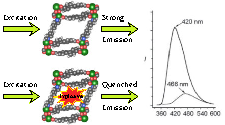
\includegraphics[width=0.7\textwidth]{figures/cited/chemical-sensor}
    \caption{Schematic representation of optical properties modifications of
    \ce{Zn2(bpdc)2(bpee)} MOF. Image adapted with permission from
    reference~\cite{Lan2009}, copyright (2009) Wiley.}
    \label{fig:chemical-sensor}
\end{figure}

Some MOFs have luminescent properties, linked either to the presence of aromatic
or functionalized linkers or a metal cation from the lanthanide group. These
luminescent properties, combined with the adsorption capabilities of MOFs open
the possibility of using MOFs as chemical sensors. The structural and/or
electronic transition of a MOF upon adsorption will modify the light emission
properties of the material, allowing to detect specific gaseous compounds. This
is have been developped in particular to detect explosive materials at low
concentrations. For example, the \ce{Zn2(bpdc)2(bpee)} MOF is able to detect
multiple nitro-substituted molecules found in explosives such as
2,4-dinitrotoluene or 2,3-dimethyl-2,3-dinitrobutane in around
\SI{10}{s}\cite{Lan2009} (see figure~\ref{fig:chemical-sensor}). Another example
is the \ce{[Zn2(oba)2(bpy)]3} MOF, also able to detect explosive and aromatic
molecules through a fluorescence quenching phenomenon\cite{Pramanik2011}.

\newpage
\section{Adsorption and intrusion}

Adsorption is an interface phenomenon, where molecules or atoms are depositing
and creating a thin film at the surface of a material. Because they have a high
specific surface area, the adsorption in porous materials is several orders of
magnitude higher than on the external surface of bulk materials. Adsorption is
used as a characterization technique for porous media, and is also the basis of
their most prevalent applications.

\subsection{Adsorption of gases}

It is possible to study adsorption both with experimental and theoretical
approaches. The central tool for the study of adsorption is the single component
adsorption isotherm. Considering a pure gas adsorbing in a porous matrix, the
adsorption isotherm records the amount of adsorbed gas (also called
\emph{loading}) at a fixed temperature as a function of the pressure $P$, or the
more commonly, the pressure relative to the vapor pressure of the gas $P/P_0$.
Experimentally, these adsorption isotherms are obtained with gravimetric,
volumetric or chromatographic methods\cite{Ruthven1984, Yang1987}.

\begin{figure}[htb]
    \centering
    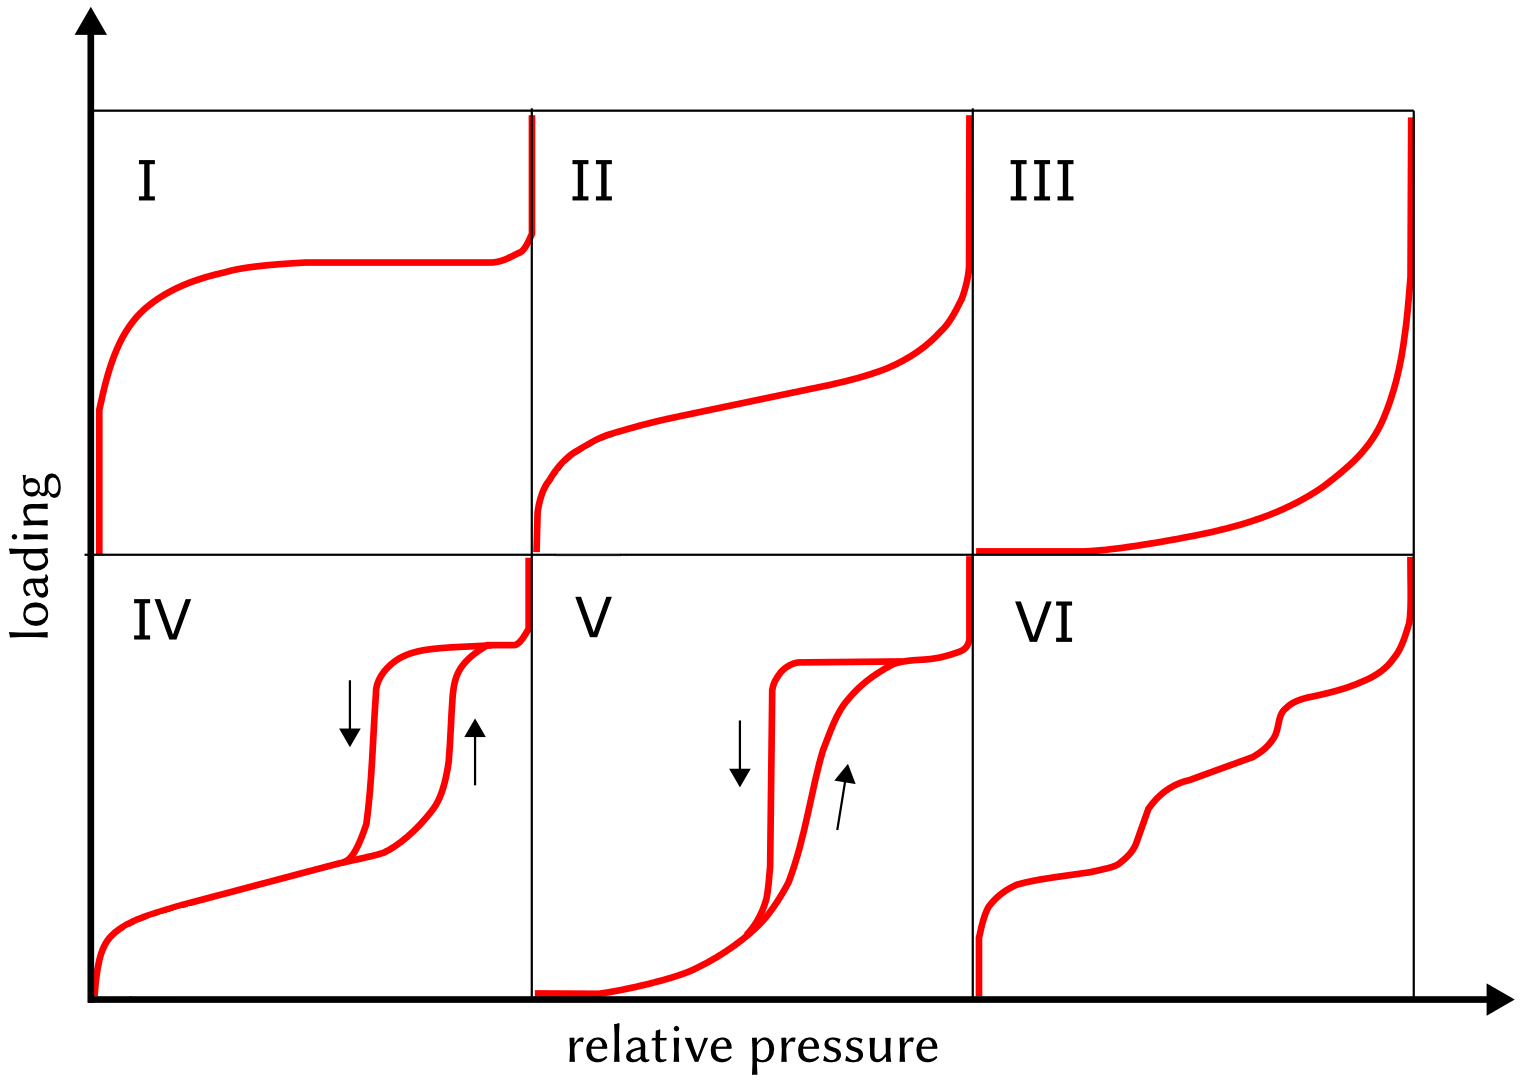
\includegraphics[width=0.75\textwidth]{figures/images/iupac-isotherms}
    \caption{IUPAC classification of isotherms.}
    \label{fig:iupac-isotherms}
\end{figure}

The IUPAC classifies adsorption isotherms depending on their shape, as
represented in figure~\ref{fig:iupac-isotherms}\cite{Sing1985}. Only the
isotherms of type I, IV and V can occur in nanoporous solids. Type I isotherms
are concave, reversible and the adsorbed quantity of matter goes to a finite
value as the pressure increases. It is the most common isotherm type, and
express the prevalence of gas--solid interactions over gas--gas interactions in
a material containing a single kind of equivalent adsorption sites.

Type IV isotherms also present a maximal loading, and one or two steps with
sometimes a hysteresis loop between the adsorption and desorption branches.
These steps are usually attributed to a modification in the structure of the
adsorbing solid\cite{Karge1989}. Type V isotherm shows an inflection point: at
low pressure the adsorption is very low, mainly due to small gas--solid
interactions. For higher pressures the adsorption becomes stronger thanks to
interactions between the gas molecule themselves. In flexible porous materials,
type IV isotherms would be associated with \emph{breathing} materials, and type
V isotherms with \emph{gate opening}. Finally, isotherms types II, III and VI do
not present a maximal loading, and are usually observed in solids with multiple
pore sizes and a continuous transition from mono-layer adsorption to
multi-layers adsorption and capillary condensation.

It is possible to study and predict adsorption isotherms using theoretical
methods such as thermodynamic models and molecular simulations methods such as
Grand Canonical Monte Carlo. I will present with more details the methods I used
during my PhD to study adsorption in the corresponding chapters:
chapter~\ref{sec:macroscopic} for macroscopic thermodynamics modeling; and
chapter~\ref{sec:molsim} for molecular simulations.

\subsection{Intrusion of liquids}

The intrusion of liquids, and in particular mercury, has been used for a long
time to characterize porous materials having pore widths in the macropore range
of \SI{50}{nm} to \SI{500}{\um}\cite{Rouquerol2011}. Intrusion can be seen as
adsorption of fluids above the vapor pressure ($P > P_0$), \ie when the fluid is
in its liquid state. A sketch of an intrusion--extrusion porosimeter is given in
figure~\ref{fig:porosimeter}. In this device, a non-wetting fluid is pressurized
and will enter the porous network at a pressure linked to the pore width $h$ by
the Washburn equation\cite{Fraux2017-2}:
\[P = \frac{2\gamma\cos\theta}{h},\]
where $\gamma$ is the surface tension of the liquid/gas interface, and $\theta$
the angle of contact along the triple line solid/liquid/gas.

\begin{figure}[htb]
    \centering
    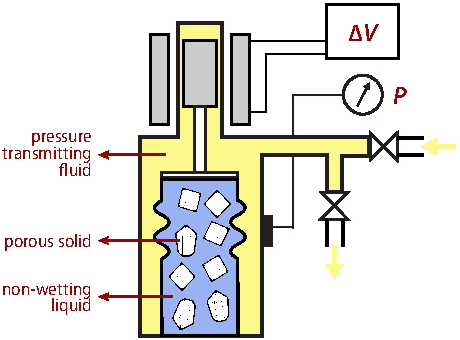
\includegraphics[width=0.7\textwidth]{figures/images/porosimeter}
    \caption{Sketch of an intrusion--extrusion porosimeter. A sample of porous
    solid powder is placed in a non-wetting liquid (in blue) and pumps control
    the pressure of a pressure-transmitting fluid (in yellow). A manometer
    records the pressure $P$ during the experiment, and a transducer records
    changes in volume of the system.}
  \label{fig:porosimeter}
\end{figure}

\newpage
In the 2000s, water was used as non-wetting fluid in an adapted porosimetry device
to characterize hydrophobic nanoporous materials such as silica
gels\cite{Fadeev1997} and siliceous zeolites\cite{Eroshenko2001, Eroshenko2002}
or micelle-templated silica\cite{Lefevre2004}. More recently, forced wetting of
electrolyte solutions was studied, disclosing very interesting giant osmotic
pressure effects\cite{Liu2009, MichelinJamois2015}. Water can only be used as a
non-wetting fluid in \emph{hydrophobic solid}, where the potential energy
interaction between the water molecules and the confining solid wall is much
weaker than the water molecules' mutual interaction. This use of water as a
non-wetting fluids opened a new field of applications for the intrusion in
nanoporous solids based on mechanical energy storage and
dissipation\cite{Eroshenko2001, Fraux2017-2}. Interested readers can consult the
review I helped to write on the subject, published in
\citejournal{Fraux2017-2}\cite{Fraux2017-2}, for more details.

The general idea of storing energy by forced intrusion of a non-wetting fluids
in porous media was first explored by \citeauthor{Fadeev1997} some years
ago\cite{Fadeev1997}. In 2001, \citeauthor{Eroshenko2001}\cite{Eroshenko2001}
reported a stepwise intrusion-extrusion isotherm of water in two different
hydrophobic zeolites, namely zeolite $\beta$ and silicalite-1 at pressures
around 60 and \SI{80}{MPa} respectively, \ie notably above the water saturation
pressure of \SI{3 500}{Pa} at room temperature.

\begin{figure}[ht]
    \centering
    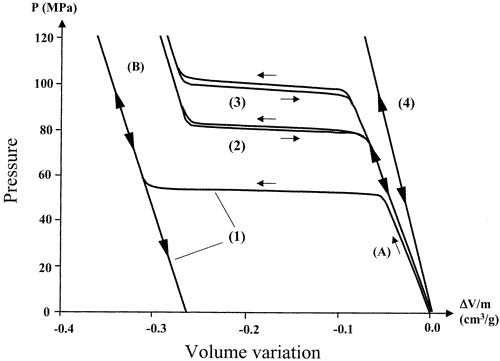
\includegraphics[width=0.75\linewidth]{figures/cited/intrusion-zeosil}
    \caption{Pressure-volume intrusion isotherms of water in (1) zeolite
    $\beta$; (2) silicalite-1 (\ce{OH-}); (3) silicalite-1 (\ce{F-}) and (4)
    Na-ZSM-5. Reprinted with permission from reference~\cite{Eroshenko2001},
    copyright (2001) American Chemical Society.}
    \label{fig:intrusion-zeosil}
\end{figure}

The reported intrusion isotherms are reproduced in
figure~\ref{fig:intrusion-zeosil}. From these results, the authors proposed that
it was possible to use these heterogeneous systems to "accumulate, restore and
dissipate mechanical energy", thus opening new routes in the field of
energetics. In terms of energy storage devices, a system displaying an
intrusion-extrusion cycle without hysteresis can simply be termed as a
\emph{spring}. A system with hysteresis is a \emph{shock absorber} and an
incomplete cycle in which water is retained in the porous framework upon
pressure release can be called a \emph{bumper} (see also the
figure~\ref{fig:intrusion-shapes} for an illustration of these behaviors).

\begin{figure}[p]
    \centering
    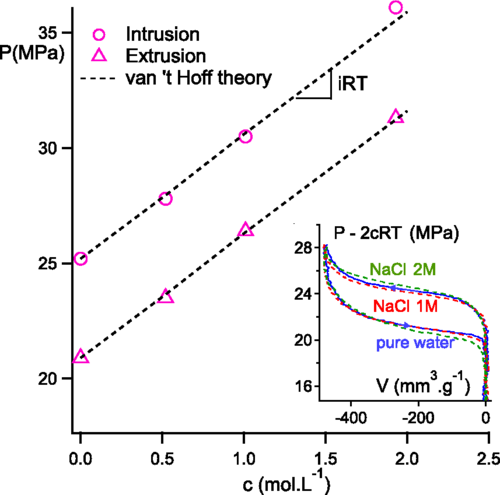
\includegraphics[width=0.6\textwidth]{figures/cited/osmotic-zif}
    \caption{Intrusion and extrusion pressures for NaCl solutions of
    various concentrations in ZIF-8 at 323 K. The inset displays
    intrusion--extrusion curves, plotted not in absolute pressure $P$ but as a
    function of $\ P - 2cRT$, showing that the effect of concentration is well
    explained by the van 't Hoff osmotic pressure. Reprinted with permission
    from reference~\cite{MichelinJamois2015}, copyright (2015) American
    Physical Society.}
    \label{fig:osmotic-zif}
\end{figure}

\begin{figure}[p]
    \centering
    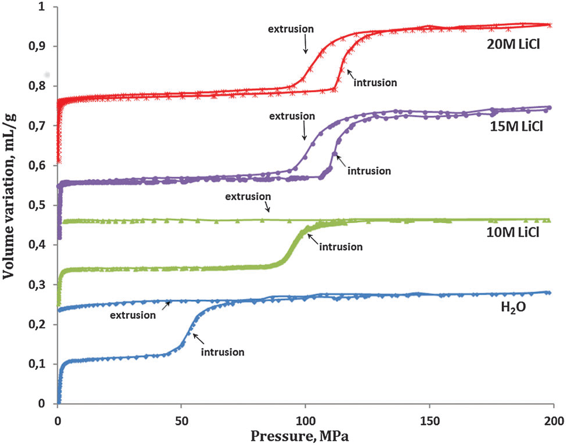
\includegraphics[width=0.7\textwidth]{figures/cited/intrusion-licl}
    \caption{Intrusion-extrusion process in $\beta$ zeosil. With pure water, it
    behaves like a bumper. As the LiCl concentration increases, the intrusion
    pressure is enhanced and a change in behavior from bumper to shock-absorber
    is observed from 10~M to 15~M of LiCl. Reproduced from
    reference~\cite{Ryzhikov2014}, with permission from the PCCP Owner Societies.}
    \label{fig:intrusion-licl}
\end{figure}

Patarin and coworkers\cite{Tzanis2014, Khay2014} were the first to show that the
intrusion pressure in silicalite-1 was increased by a factor of 3 when using a
concentrated solution of lithium chloride, instead of pure water. Consequently,
the stored energy was also increased by the same factor, which seems very
promising in view of potential energy storage applications. This has lead to a
number of such aqueous solutions intrusion-extrusion studies in various zeosils
as well as hydrophobic ZIF materials. In addition to the effect of increasing
the intrusion pressure, the use of electrolyte solutions can lead to a drastic
change in the intrusion-extrusion behavior.
\citeauthor{Ryzhikov2014}\cite{Ryzhikov2014} showed that $\beta$-zeosil changed
its behavior from bumper to shock-absorber, as the LiCl concentration increased
from \SI{10}{mol/L} to \SI{15}{mol/L}. This is shown in
figure~\ref{fig:intrusion-licl}.

Intrusion of electrolyte solutions in \ZIF8 was recorded using several
concentrations and different electrolytes\cite{Ortiz2014, MichelinJamois2015}.
In all cases, the intrusion pressure increased as the electrolyte concentration
increased and the intrusion-extrusion cycles were shifted replicas of the pure
water cycles. Based on the findings of a molecular dynamics study\cite{Hu2011},
Michelin-Jamois suggested that only pure water was intruded in the material's
pore. According to this hypothesis, the shift in intrusion pressure is due to
the osmotic pressure, \ie the difference in pressure between the pure water
pressure inside the pore and the aqueous solution pressure outside the porous
framework. A simple application of the van't Hoff osmotic equation ($\Pi = i c R
T$) confirmed this model in most of the studied cases, as illustrated in
figure~\ref{fig:osmotic-zif}.

Even more recently, \citeauthor{Arletti2016}\cite{Arletti2016} coupled
intrusion-extrusion experiments of \ce{MgCl2} aqueous solution to \emph{in situ}
high-pressure synchrotron X-ray diffraction analysis. This study clearly
demonstrated the presence of both ions and water molecules in the high pressure
intruded liquid. During my PhD, I approached the question of when and why ions
in the aqueous solution enter the microporous frameworks using classical
molecular simulations, the corresponding work is presented in
chapter~\ref{sec:classical}.

\begin{figure}[b]
    \centering
    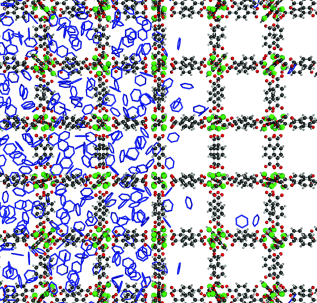
\includegraphics[width=\textwidth]{figures/cited/mof5-bezene}
    \caption{Snapshots of molecular dynamics simulations of benzene in MOF-5 at
    (a) \SI{125}{K} and (b) \SI{50}{K}. At \SI{50}{K}, vapor–liquid coexistence
    takes place, the vapor and liquid phases extending over many unit cells.
    Adapted with permission from reference~\cite{Braun2015}, copyright (2015)
    Wiley.}
    \label{fig:mof5-bezene}
\end{figure}

\clearpage

\subsection{Coupling adsorption and deformations}

Adsorption and intrusion in flexible nanoporous materials can present very
interesting behaviors. First, some materials deforms during adsorption, creating
the aforementioned effects of breathing, gate opening or even negative gas
adsorption\cite{Krause2016}. At the same time, because they are constrained by
the surrounding porous solid, fluids inside the pores adopt different static
organization and dynamic behavior than fluids in the bulk state. These effects
of the porous solids on the fluids are grouped together under the category of
\emph{confinement} effects.

Confinement effects introduce another way to look at adsorption and intrusion:
two different phases of the same chemical species are at equilibrium, and
transfers from one phase to the other occurs as the fluid enters or leave the
porous structure. In some cases, there can even be multiple different fluid
phases inside the porous volume. Recently,
\citeauthor{Braun2015}\cite{Braun2015} demonstrated, using NMR relaxometry and
molecular dynamics, that a true liquid–vapor coexistence existed in fluid
benzene confined in MOF-5. The liquid and vapor phases were shown to extend over
many unit cells thanks to the open 3D framework, as shown in
figure~\ref{fig:mof5-bezene}.

While confinement effects also occurs in rigid nanoporous material, when working
with flexible nanoporous materials we need to consider multiple phases
equilibrium occurring at the same time. The fluid phase equilibrium between the
bulk state and the confined state can have an influence on phase equilibrium
between the porous material phases and reciprocally.

During my PhD work, I explored confinement effects mainly in \ZIF8, with
different fluids: gaseous nitrogen at \SI{77}{K} in chapter~\ref{sec:ab-initio},
and aqueous solutions at ambient temperature in chapter~\ref{sec:classical}. I
also looked at more rigid systems --- namely aluminosilicate nanotubes --- in
chapter~\ref{sec:imogolites}. I have been particularly interested in the
simulation methods one can use to study the coupling between adsorption and
deformations in flexible nanoporous materials.
\newpage

\OnlyInSubfile{\printglobalbibliography}

\end{document}
